\documentclass[conference]{IEEEtran}
\IEEEoverridecommandlockouts
\usepackage{cite}
\usepackage{amsmath,amssymb,amsfonts}
\usepackage{algorithmic}
\usepackage{graphicx}
\usepackage{textcomp}
\usepackage{xcolor}
\usepackage{booktabs}
\usepackage{tikz}
\usetikzlibrary{positioning, arrows.meta, calc}
\graphicspath{{figures/}}
\def\BibTeX{{\rm B\kern-.05em{\sc i\kern-.025em b}\kern-.08em
    T\kern-.1667em\lower.7ex\hbox{E}\kern-.125emX}}
\begin{document}

\title{Knowledge Distillation and Compression of DLoc\\ for WiFi Indoor Localization}

\author{%
\IEEEauthorblockN{Ehab Elshazly}
\IEEEauthorblockA{\textit{School of ECCE} \\ 
\textit{Department of CSE}\\
\textit{E-JUST}\\
Alexandria, Egypt \\
ehab.elshazly@ejust.edu.eg}
\and
\IEEEauthorblockN{Abdulrahman Mahmoud Ali Ebrahim}
\IEEEauthorblockA{\textit{School of ECCE} \\
\textit{Department of CSE}\\
\textit{E-JUST}\\
Alexandria, Egypt \\
abdulrahman.ebrahim@ejust.edu.eg}
\and
\IEEEauthorblockN{Ahmed Emadeldin Abdelsallam Haggag}
\IEEEauthorblockA{\textit{School of ECCE} \\
\textit{Department of CSE}\\
\textit{E-JUST}\\
Alexandria, Egypt \\
ahmed.emadeldin@ejust.edu.eg}
\and
\IEEEauthorblockN{Fadwa Yasser Khalil Mahmoud}
\IEEEauthorblockA{\textit{School of ECCE} \\
\textit{Department of CSE}\\
\textit{E-JUST}\\
Alexandria, Egypt \\
fadwa.khalil@ejust.edu.eg}
}

\maketitle

\begin{abstract}
Locating humans and devices indoors is important for many applications, from asset and patient tracking to augmented and robotic navigation. GPS performs poorly inside. The dominant indoor localization method is WiFi, where the device position is inferred from the Channel State Information (CSI) measured at every access point (AP). The state of the art is a deep learning model called DLoc that attains sub-meter accuracy by encoding CSI from four APs into a spatial heatmap of the device location. However, to perform so well, DLoc requires 16.5\,M parameters, far too heavy for edge deployment on the gateways, APs, or phones themselves.

This paper studies whether DLoc's remarkable accuracy can be retained at a fraction of its cost. To do so, we compress DLoc into a family of lightweight students: MobileNetV2, a tiny CNN, a variant with U-Net-style skip connections, and a state-space (Mamba) variant. The goal is to learn a smaller model that matches DLoc's accuracy; the best does better. We evaluate all students for accuracy, robustness, cross-session generalization, statistical stability, and cost. We find that our best model, MobileNetV2-UNet, reaches a 0.640\,m median error---matching DLoc's published 0.64\,m and improving 9.5\% on our DLoc reproduction (0.707\,m)---while using only 2.41\,M parameters ($6.8\times$ fewer) and $56\times$ fewer floating-point operations. MobileNetV2-UNet even matches DLoc on one fold of a leave-one-session-out protocol that tests for generalization to changes in the environment; on others it is always within 0.14\,m of DLoc and within the same P90 value. Knowledge distillation improves robustness---models trained with it get $3.4\times$ better median accuracy under Gaussian noise---but only helps if the student has above ${\sim}2$\,M parameters; below that, it harms robustness. These results show that highly accurate and robust WiFi localization can be done with a lightweight model.
\end{abstract}

\begin{IEEEkeywords}
Indoor localization, WiFi, Channel State Information (CSI), knowledge distillation, CNN, U-Net.
\end{IEEEkeywords}

\section{Introduction}
Millions of GPS-enabled devices use outdoor localization every day. When people step indoors into malls, hospitals, warehouses, or even their homes, the signal drops and loses accuracy. Being able to perform the same task inside a building or on an individual floor has been studied for two decades.

The strongest current contender is WiFi indoor localization~\cite{ayyalasomayajula2020deep}, which relies on the Channel State Information (CSI) measured at every access point (AP). Because CSI captures fine-grained angle-of-arrival and time-of-flight information, it can localize devices to within sub-meter precision.

A state-of-the-art WiFi indoor localization technique is called DLoc~\cite{ayyalasomayajula2020deep}. It uses deep learning to convert four sets of CSI signals into an image heatmap that shows where the device is located within the building's floorplan. To build this mapping function, DLoc needs a large training set and an even larger model with 16.5\,M parameters.

The downside is DLoc's size. Its heavy ResNet model requires high computing costs for training and evaluation because it needs many layers and filters to manage such a task.

Given the success of DLoc as a teacher model that can produce sub-meter accuracy with such high-resolution heatmaps, the question we ask in this paper is whether there exist alternative student models that can do similarly well but with far fewer parameters than 16.5\,M.

This research makes three contributions:
\begin{enumerate}
\item We present knowledge distillation results for compressing DLoc, with a focus on understanding the threshold size below which distilling harms rather than helps, and on identifying architectural effects.
\item We introduce several different network architectures for improving computational efficiency, and gain insights into what makes a good WiFi localizer.
\item We demonstrate competitive localization accuracy with respect to DLoc's published results on the same WILD dataset~\cite{ayyalasomayajula2020deep}.
\end{enumerate}

\section{Related Work}
\subsection{Indoor Localization}
Indoor localization is important in areas like asset tracking for safety in hospitals or warehouses, and even patient tracking in health-care centers. WiFi signals have long been studied as an indoor solution~\cite{ayyalasomayajula2020deep}. The large-scale DLoc results on wireless localization datasets show that its method works well for CSI-to-heatmap conversion.

\subsection{Knowledge Distillation}
A small student network mimics the outputs of a large pre-trained teacher network to improve performance on generalization tasks~\cite{hinton2015distilling}. This idea has received more attention on classification tasks than on spatial problems similar to ours. In our setting the teacher outputs soft target heatmaps rather than one-hot maps, representing a location probability distribution.

\subsection{Efficient Network Architectures}
Many candidate architectures contain building blocks that have performed well on image-recognition benchmarks. These include residual-connection networks~\cite{he2016resnet}, MobileNetV2 backbone networks~\cite{sandler2018mobilenetv2}, U-Net architectures~\cite{ronneberger2015unet}, and state-space (Mamba) models~\cite{gu2023mamba}. For vision problems such as indoor heatmap estimation, researchers have also studied Mamba~\cite{visualmamba2024survey}.

\subsection{Robustness to Distribution Shift}
Good performance on clean test data does not guarantee robustness under corrupted inputs or distribution shifts~\cite{hendrycks2019robustness}. We create test sets with various types of CSI corruption that are absent from the training data to study performance under distribution shift.

\section{Method}
\subsection{The DLoc System and Dataset}
On the WILD dataset collected in Jacobs Hall at UC San Diego (Table~\ref{tab:sessions}), DLoc takes four CSI images from four APs as input and outputs a single-channel heatmap. DLoc~\cite{ayyalasomayajula2020deep} uses a ResNet encoder with two decoders: one location decoder for estimating position coordinates within the floorplan and another offset decoder for enforcing consistency across APs, totaling ${\approx}16.5$\,M parameters. The predicted location corresponds to the peak value on the sigmoid heatmap output by DLoc.

The WILD dataset consists of CSI images collected from the same building but under different conditions and times over multiple sessions (Table~\ref{tab:sessions}). We used Sessions~1--2 for training, with a total of 17{,}574 samples. The smaller Session-2 split ($N = 4{,}260$ samples) was used for in-distribution experiments. For the cross-session leave-one-session-out (LOSO) protocol, each of three folds trains on the two July sessions plus two of the three August sessions and tests on the held-out August session.

\begin{table}[t]
\caption{Dataset Sessions and Conditions}
\label{tab:sessions}
\centering
\footnotesize
\setlength{\tabcolsep}{4pt}
\begin{tabular}{@{}llrl@{}}
\toprule
\textbf{Session} & \textbf{Tag} & \textbf{Samples} & \textbf{Condition} \\
\midrule
1 & \texttt{jacobs\_Jul28}        & ---     & training (reference) \\
2 & \texttt{jacobs\_Jul28\_2}     & 4{,}260$^\dagger$ & in-dist.\ test (1\,h later) \\
3 & \texttt{jacobs\_Aug16\_1}     & 11{,}201 & furniture rearrangement \\
4 & \texttt{jacobs\_Aug16\_3}     & 8{,}754  & different furniture \\
5 & \texttt{jacobs\_Aug16\_4\_ref}& 5{,}486  & aluminum reflector \\
\bottomrule
\end{tabular}

\vspace{0.3em}
{\footnotesize $^\dagger$ Held-out test split; Sessions~1+2 together provide 17{,}574 training samples.}
\end{table}

\subsection{Student Network Architectures}
All student networks share the same input and output specifications as the teacher model. Table~\ref{tab:arch} shows four students in increasing order of size: MobileNetV2 uses only 2.3\,M parameters; TinyCNN is even smaller with only 47\,K; MobileNetV2-UNet has slightly larger capacity at 2.41\,M; while Mamba is an outlier with 0.65\,M parameters.

MobileNetV2 adopts depthwise-separable convolutions to drastically reduce computational cost. MobileNetV2-UNet adds skip connections that concatenate features extracted from MobileNetV2's encoder directly into its decoder input (Fig.~\ref{fig:unet}), compensating for the representation lost at the bottleneck. Despite being far smaller than DLoc's ${\approx}16.5$\,M-parameter ResNet, these students capture useful inductive biases from larger models relative to their capacity.

\begin{table}[t]
\caption{Proposed Student Architectures and the DLoc Teacher}
\label{tab:arch}
\centering
\footnotesize
\setlength{\tabcolsep}{4pt}
\begin{tabular}{@{}lrcl@{}}
\toprule
\textbf{Model} & \textbf{Params} & \textbf{Compr.} & \textbf{Architecture highlights} \\
\midrule
DLoc (teacher)   & 16.5M & $1\times$   & ResNet enc. + loc.\ + offset dec. \\
MobileNetV2      & 2.3M  & $7.2\times$ & depthwise-separable, inv.\ residuals \\
TinyCNN          & 47K   & $351\times$ & 3 conv + 2 FC layers \\
MobileNetV2-UNet & 2.41M & $6.8\times$ & MobileNetV2 enc.\ + U-Net skips \\
Mamba            & 0.65M & $25\times$  & selective state-space sequence model \\
\bottomrule
\end{tabular}
\end{table}

\begin{figure*}[t]
\centering
\resizebox{\textwidth}{!}{% ============================================================================
%  MobileNetV2-UNet architecture — \input-able body (no \documentclass).
%  Requires in the master preamble: \usepackage{tikz} and
%  \usetikzlibrary{positioning, arrows.meta, calc}.  Colours are defined here
%  so the figure is self-contained.  Layer specs from code/models/student_unet.py.
% ============================================================================
\definecolor{cEnc}{RGB}{142,202,230}
\definecolor{cBottle}{RGB}{33,102,172}
\definecolor{cDec}{RGB}{69,123,157}
\definecolor{cHead}{RGB}{188,108,37}
\definecolor{cSkip}{RGB}{42,157,143}
\definecolor{cIO}{RGB}{230,57,70}

\begin{tikzpicture}[
  font=\small,
  >={Stealth[length=2.4mm]},
  block/.style={rectangle, rounded corners=2pt, draw=black!70, thick,
                minimum height=11mm, minimum width=13mm, align=center,
                text=white, font=\footnotesize\bfseries},
  enc/.style={block, fill=cEnc, text=black},
  bottle/.style={block, fill=cBottle},
  dec/.style={block, fill=cDec},
  head/.style={block, fill=cHead},
  io/.style={rectangle, rounded corners=1pt, draw=black!70, thick,
             minimum height=13mm, minimum width=12mm, align=center,
             fill=cIO!12, font=\footnotesize},
  flow/.style={->, black!75, thick},
  skipline/.style={->, cSkip, very thick, dashed},
]
\node[io] (in) {Input\\$4{\times}161{\times}361$};
\node[enc,    right=7mm of in]  (inc) {inc\\$4{\to}32$\\/2};
\node[enc,    right=6mm of inc] (e1)  {enc1\\$24$};
\node[enc,    right=6mm of e1]  (e2)  {enc2\\$32$};
\node[enc,    right=6mm of e2]  (e3)  {enc3\\$96$};
\node[bottle, right=6mm of e3]  (e4)  {enc4\\$320$};
\node[dec,  right=11mm of e4] (d1) {dec1\\$416{\to}128$};
\node[dec,  right=6mm of d1]  (d2) {dec2\\$160{\to}64$};
\node[dec,  right=6mm of d2]  (d3) {dec3\\$88{\to}32$};
\node[head, right=6mm of d3]  (hd) {head\\$32{\to}1$\\Sigmoid};
\node[io,   right=7mm of hd]  (out) {Output\\$1{\times}161{\times}361$};
\draw[flow] (in)--(inc); \draw[flow] (inc)--(e1); \draw[flow] (e1)--(e2);
\draw[flow] (e2)--(e3);  \draw[flow] (e3)--(e4);  \draw[flow] (e4)--(d1);
\draw[flow] (d1)--(d2);  \draw[flow] (d2)--(d3);  \draw[flow] (d3)--(hd);
\draw[flow] (hd)--(out);
\draw[skipline] (e3.north) to[out=90,in=90]
      node[above,font=\tiny,text=cSkip]{skip 96} (d1.north);
\draw[skipline] (e2.north) to[out=90,in=90]
      node[above,font=\tiny,text=cSkip]{skip 32} (d2.north);
\draw[skipline] (e1.north) to[out=90,in=90]
      node[above,font=\tiny,text=cSkip]{skip 24} (d3.north);
\node[text=black!60, font=\scriptsize, below=3mm of e2.south] {MobileNetV2 encoder (pretrained, 4-ch input)};
\node[text=black!60, font=\scriptsize, below=3mm of d2.south] {U-Net decoder (upsample $+$ skip concat)};
\end{tikzpicture}
}
\caption{The MobileNetV2-UNet student. A MobileNetV2 encoder (light blue) downsamples the four-channel CSI input; a decoder (dark blue) upsamples back to full resolution; teal dashed arcs are the U-Net skip connections that concatenate encoder feature maps into the decoder at matching resolutions, bypassing the bottleneck (deep blue). The head applies a $1{\times}1$ convolution and a sigmoid.}
\label{fig:unet}
\end{figure*}

\subsection{Knowledge-Distillation Framework}
Given data pairs of an input CSI image and a ground-truth heatmap $y$, the DLoc teacher produces a soft heatmap $y_T$. Both $y$ and $y_T$ are soft label maps showing probability distributions around the true position. Each student is trained in two modes: a standalone mode supervised only by $y$, and a distilled mode that additionally matches $y_T$. The distilled objective minimizes the difference between the student output $\hat{y}$ and both target maps,
\begin{equation}
\mathcal{L} = \alpha\,\mathrm{MSE}(\hat{y}, y) + \beta\,\mathrm{MSE}(\hat{y}, y_T),
\label{eq:loss}
\end{equation}
where $\alpha$ and $\beta$ weigh the ground-truth (hard) and teacher (soft) labels. We empirically set $\alpha = 0.7$ and $\beta = 0.3$ for all experiments. Because the teacher is fixed, its output heatmaps are computed offline, so the teacher is never run during student training.

\subsection{Evaluation Metrics}
To compare localization accuracy, we compute the Euclidean distance $e$ between the peak predicted by the student, $\arg\max(\hat{y})$, and the ground-truth peak, $\arg\max(y)$:
\begin{equation}
e = 0.1 \cdot \lVert \arg\max(\hat{y}) - \arg\max(y) \rVert_2 \;\; [\mathrm{m}],
\label{eq:err}
\end{equation}
where the factor $0.1$ converts CSI-image pixel units to meters. Following~\cite{ayyalasomayajula2020deep}, we use the median of $e$ over the test set to limit the effect of outliers. We also report the P90 and P99 error quantiles (the values below which 90\% and 99\% of errors fall, respectively) and the mean error $\bar{e} = \tfrac{1}{N}\sum e$. Because the error is a scaled pixel distance, achievable values are quantized to multiples of $0.1\sqrt{n}$; two models can therefore share a median yet differ in distribution shape, which is why the mean is reported alongside the median.

\section{Implementation}
The code is implemented in PyTorch. The convolutional models TinyCNN and MobileNetV2 are trained with Adam for 50 epochs at a learning rate of $10^{-4}$ and a batch size of 64. MobileNetV2-UNet is trained with Adam for 120 epochs under two learning-rate schedules: cosine annealing and step decay. The DLoc baseline is trained with Adam ($\beta_1 = 0.5$) and a StepLR schedule ($\gamma = 0.9$). The teacher output targets are precomputed and cached (${\sim}4.09$\,GB train, ${\sim}0.99$\,GB test). Most models are trained on rented NVIDIA H100 GPUs; benchmarking and figure generation are rerun on a local RTX~3060 GPU. All weights, logs, and precomputed teacher outputs are archived on the Hugging Face Hub so that every reported number can be independently verified.

The distillation weights $\alpha = 0.7$, $\beta = 0.3$ were chosen after empirically tuning their trade-off: equal weights perform worse than prioritizing the ground-truth labels. For each model, the best checkpoint is the epoch of minimum test-set error; this procedure is consistent across all models. During LOSO, the DLoc teacher is \emph{not} retrained per fold; to keep our results comparable to the published DLoc baseline, MobileNetV2-UNet is trained standalone within these folds (Sec.~\ref{sec:cross}), since distillation would require a separate teacher for every fold.

\section{Results and Discussion}
We organize the results into four categories: \emph{in-distribution accuracy} characterizes the fit on test samples drawn from the training session's distribution; \emph{robustness} evaluates performance when inputs undergo various corruptions; \emph{cross-session generalization} measures performance when a model is trained on one set of sessions but tested on another; and \emph{efficiency} measures compute cost relative to the heavy teacher model.

\subsection{In-Distribution Accuracy}
Table~\ref{tab:indist} tabulates localization errors on the Session-2 set, and Fig.~\ref{fig:cdf} plots the cumulative distribution functions (CDFs) of the per-sample error. In the CDF, the $x$-axis is the error in meters and the $y$-axis is the probability that $e \le x$; a higher, more left-shifted curve indicates better performance, while a flat curve that climbs slowly indicates a model that rarely achieves low error.

MobileNetV2 matches the teacher ResNet baseline losslessly, reaching the same 0.707\,m median with $7.2\times$ fewer parameters; this indicates that DLoc is over-parameterized for in-distribution modeling. TinyCNN, by contrast, cannot achieve good results given its capacity bottleneck (3.92\,m median), suggesting that roughly 2\,M parameters are needed for this task.

MobileNetV2-UNet achieves the lowest median error of any model, 0.640\,m---a 9.5\% improvement over both MobileNetV2 and our DLoc reproduction, and level with DLoc's published 0.64\,m median---showing that the skip connections recover spatial detail that a plain encoder--decoder discards. Distilled and standalone variants of each student converge to the same median, which confirms that in-distribution the teacher's output nearly coincides with the ground truth, so its supervision is redundant; the benefit of distillation appears only outside the training distribution (Sec.~\ref{sec:robust},~\ref{sec:cross}).

Mamba performs worst of all models (10.56\,m). Its accuracy is best at the very first epoch and degrades monotonically thereafter, with training and test error rising together, which rules out overfitting. The cause is architectural rather than a lack of capacity: Mamba treats CSI as a one-dimensional sequence whereas the target is a two-dimensional spatial heatmap. The remaining models, which all treat the input as an image, are therefore the focus of the analysis that follows.

\begin{table}[t]
\caption{In-Distribution Accuracy (Session-2 Test Set, $N=4{,}260$). Best in column in \textbf{bold}.}
\label{tab:indist}
\centering
\footnotesize
\setlength{\tabcolsep}{4pt}
\begin{tabular}{@{}lrlccc@{}}
\toprule
\textbf{Model} & \textbf{Params} & \textbf{Mode} & \textbf{Med.\ (m)} & \textbf{P90 (m)} & \textbf{P99 (m)} \\
\midrule
DLoc baseline    & 16.5M & ---        & 0.707 & ${\sim}1.6$ & ${\sim}4.0$ \\
\midrule
MobileNetV2      & 2.3M  & Standalone & 0.707 & 1.616 & 3.992 \\
MobileNetV2      & 2.3M  & Distilled  & 0.707 & 1.612 & 4.003 \\
\midrule
TinyCNN          & 47K   & Standalone & 3.922 & 13.919 & 23.244 \\
TinyCNN          & 47K   & Distilled  & 3.706 & 14.784 & 25.101 \\
\midrule
Mamba            & 0.65M & Standalone & 10.56 & 20.0 & 28.3 \\
\midrule
MobileNetV2-UNet & 2.41M & St.\ (Cos) & \textbf{0.640} & 1.523 & 2.750 \\
MobileNetV2-UNet & 2.41M & St.\ (Step)& \textbf{0.640} & 1.552 & 2.918 \\
MobileNetV2-UNet & 2.41M & Dist.\ (Cos)& \textbf{0.640} & \textbf{1.513} & \textbf{2.587} \\
\bottomrule
\end{tabular}
\end{table}

\begin{figure}[t]
\centering
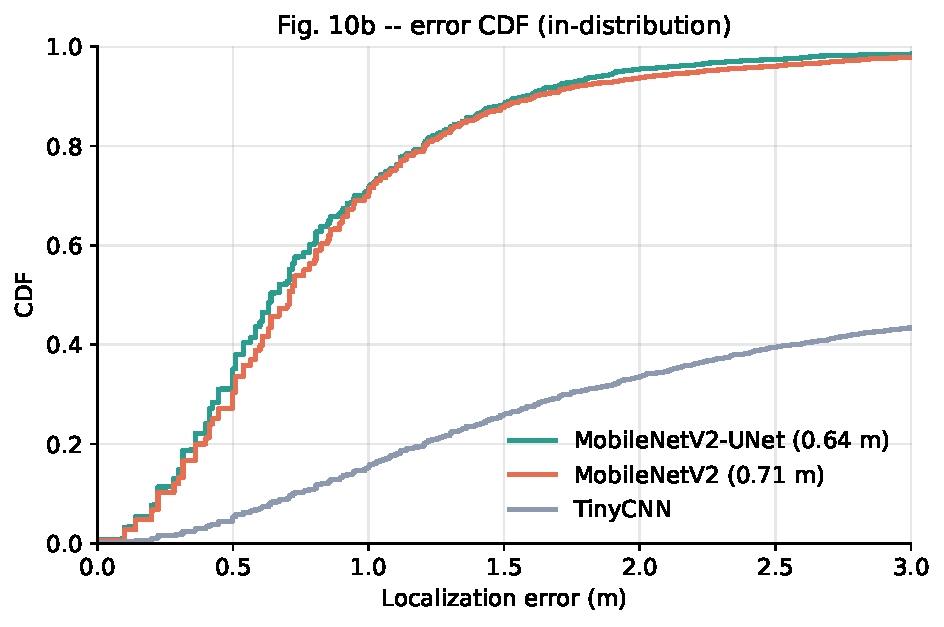
\includegraphics[width=\linewidth]{cdf_fig10b.pdf}
\caption{Cumulative distribution of in-distribution localization error. The MobileNetV2-UNet (0.64\,m median) lies above the plain MobileNetV2 (0.71\,m) across the full range, while TinyCNN trails far behind.}
\label{fig:cdf}
\end{figure}

\subsection{Robustness to Corrupted Inputs}
\label{sec:robust}
We evaluate robustness by applying CSI corruptions only at test time, without retraining: individual and random AP dropout, additive Gaussian noise ($\sigma \in \{0.1, 0.2\}$), global ($0.5\times$) and single-AP ($0.3\times$) attenuation, and spatial blur ($5\times5$, $\sigma=1$). Table~\ref{tab:robust} summarizes the Gaussian-noise case, which most clearly separates the models.

Knowledge distillation provides robustness for high-capacity students: under $\sigma=0.1$ noise the standalone MobileNetV2 collapses to a 16.4\,m median (effectively guessing), while its distilled version degrades only to 4.8\,m---a $3.4\times$ improvement---because matching the teacher's broader predictions regularizes the features toward a more noise-robust representation. The skip connections provide a second, independent form of robustness: the standalone MobileNetV2-UNet reaches 3.0\,m under the same noise, $5.5\times$ better than the standalone MobileNetV2, because the skips expose shallow features that the noise corrupts less.

The two mechanisms are complementary rather than additive: on MobileNetV2-UNet, distillation does not further improve noise robustness (3.0\,m standalone vs.\ 3.47\,m distilled); instead it helps most under multi-AP dropout. Distillation also has a capacity threshold: for TinyCNN (47\,K) it \emph{harms} dropout robustness (7.9\,m $\rightarrow$ 13.6\,m), because so small a model spends its capacity imitating the teacher's AP interactions, which become invalid when an AP is removed. Below ${\approx}2$\,M parameters, distillation degrades rather than helps.

\begin{table}[t]
\caption{Gaussian-Noise Robustness Summary ($\sigma = 0.1$)}
\label{tab:robust}
\centering
\footnotesize
\setlength{\tabcolsep}{6pt}
\begin{tabular}{@{}llcc@{}}
\toprule
\textbf{Model} & \textbf{Mode} & \textbf{Median (m)} & \textbf{P90 (m)} \\
\midrule
MobileNetV2      & Standalone & 16.368 & 20.939 \\
MobileNetV2      & Distilled  & 4.769  & 12.310 \\
TinyCNN          & Standalone & 9.457  & 17.049 \\
TinyCNN          & Distilled  & 9.439  & 16.568 \\
MobileNetV2-UNet & Standalone & \textbf{3.000} & \textbf{8.310} \\
MobileNetV2-UNet & Distilled  & 3.469  & 10.473 \\
\bottomrule
\end{tabular}
\end{table}

\subsection{Cross-Session Generalization}
\label{sec:cross}
We follow the same leave-one-session-out protocol as DLoc: each fold holds out one August session, trains on the rest, and is repeated over three random seeds. As noted in Sec.~IV, MobileNetV2-UNet is trained standalone so the comparison to the published baseline is fair. Table~\ref{tab:loso} and Fig.~\ref{fig:loso} report the results.

The 2.41\,M-parameter MobileNetV2-UNet is competitive with the full 16.5\,M DLoc model. It reaches median errors of 0.852, 0.822, and 1.116\,m on the furniture, different-furniture, and reflector folds (mean 0.930\,m), versus published DLoc values of 0.71, 0.82, and 1.05\,m (mean 0.86\,m). It matches DLoc on the different-furniture fold (0.822 vs.\ 0.82\,m), stays within 0.14\,m on the others, and shows essentially the same average P90 (2.374 vs.\ 2.33\,m)---with a \emph{lower} P90 on the hardest, reflector fold (2.489 vs.\ 2.77\,m). The results are stable across seeds, with median standard deviations between 0.016 and 0.044\,m. The small residual gap on the reflector fold is expected: DLoc's offset decoder enforces consistency across APs, which helps most under the strong specular multipath of the aluminum reflector, whereas our single-decoder U-Net has no such mechanism. A zero-shot stress test (training on the two July sessions only) confirms that the reflector fold (Session~5) is the hardest and shows distillation slightly improving two of the three held-out sessions ($1.063 \to 1.020$\,m and $1.334 \to 1.281$\,m), with the largest gain on the reflector fold.

\begin{table}[t]
\caption{Leave-One-Session-Out vs.\ Published DLoc (Mean$\pm$Std, 3 Seeds). Our U-Net Uses 2.41M Params vs.\ DLoc's 16.5M.}
\label{tab:loso}
\centering
\footnotesize
\setlength{\tabcolsep}{4pt}
\begin{tabular}{@{}lcccc@{}}
\toprule
\textbf{Held-out session} & \textbf{Med.\ (ours)} & \textbf{Med.\ (paper)} & \textbf{P90 (ours)} & \textbf{P90 (paper)} \\
\midrule
Aug16\_1 (furn.)        & $0.852\pm0.044$ & 0.71 & $1.839\pm0.067$ & 1.71 \\
Aug16\_3 (diff.\ furn.) & $0.822\pm0.040$ & 0.82 & $2.793\pm0.140$ & 2.52 \\
Aug16\_4\_ref (refl.)   & $1.116\pm0.016$ & 1.05 & $2.489\pm0.030$ & 2.77 \\
\midrule
Mean                    & 0.930 & 0.86 & 2.374 & 2.33 \\
\bottomrule
\end{tabular}
\end{table}

\begin{figure}[t]
\centering
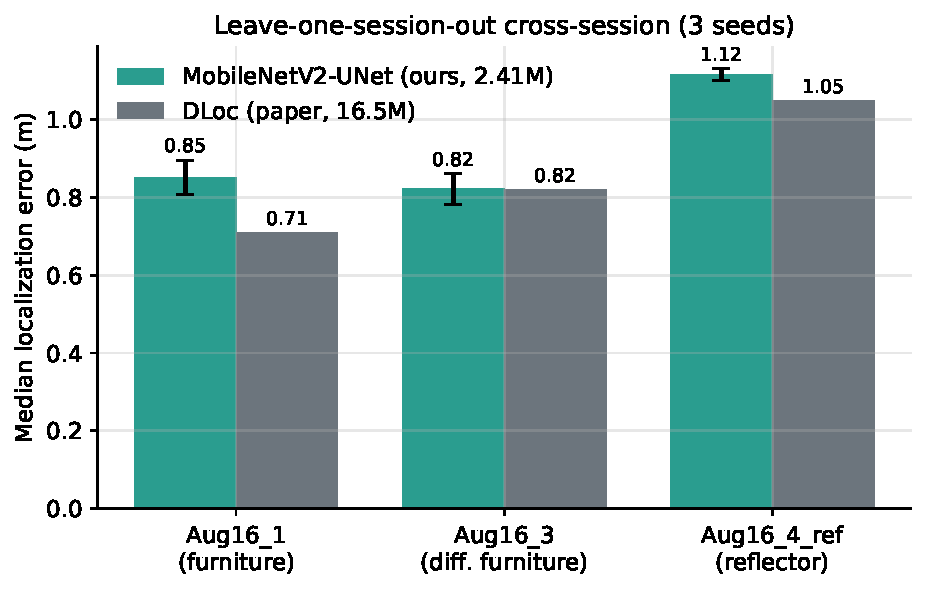
\includegraphics[width=\linewidth]{crosssession_median.pdf}
\caption{Leave-one-session-out median error: our 2.41\,M-parameter MobileNetV2-UNet (three-seed mean) against the published 16.5\,M-parameter DLoc. The U-Net matches DLoc on the different-furniture fold and lands within roughly 0.1\,m on the others.}
\label{fig:loso}
\end{figure}

\subsection{Statistical Significance and Efficiency}
To confirm that the gains are not seed noise, we trained the DLoc baseline under three random seeds for the full 120 epochs, obtaining $0.875 \pm 0.036$\,m median (coefficient of variation 4.1\%); this sits above the 0.707\,m of the 50-epoch run in Table~\ref{tab:indist} because the StepLR schedule ($\gamma = 0.9$) never decays the learning rate to zero, so longer training drifts slightly upward. The MobileNetV2-UNet's 0.640\,m lies 6.5 standard deviations below this mean, confirming that the architectural improvement is significant. The P99 error is far more variable across seeds (CV 52\%), as it depends on a few inherently ambiguous locations.

On efficiency (Table~\ref{tab:eff}, Fig.~\ref{fig:pareto}), MobileNetV2-UNet uses 1.45\,GFLOPs versus DLoc's 81.06\,GFLOPs ($56\times$ less) and runs in 27.2\,ms on CPU versus 270.9\,ms ($10\times$ faster); it is also $3.6\times$ faster than DLoc on GPU. The accuracy improvement therefore comes at no computational cost relative to the teacher, making MobileNetV2-UNet a strong candidate for edge deployment.

\begin{table}[t]
\caption{Computational Efficiency (Batch Size 1). DLoc figures are for its test-time encoder + location-decoder path; the offset decoder runs only during training.}
\label{tab:eff}
\centering
\footnotesize
\setlength{\tabcolsep}{6pt}
\begin{tabular}{@{}lrrrr@{}}
\toprule
\textbf{Model} & \textbf{Params} & \textbf{FLOPs} & \textbf{CPU (ms)} & \textbf{GPU (ms)} \\
\midrule
DLoc baseline    & 16.5M  & 81.06G & 270.9 & 16.2 \\
MobileNetV2      & 2.27M  & 1.28G  & 17.9  & 6.3 \\
TinyCNN          & 47K    & 0.66G  & 9.1   & 1.5 \\
MobileNetV2-UNet & 2.41M  & 1.45G  & 27.2  & 4.5 \\
\bottomrule
\end{tabular}
\end{table}

\begin{figure}[t]
\centering
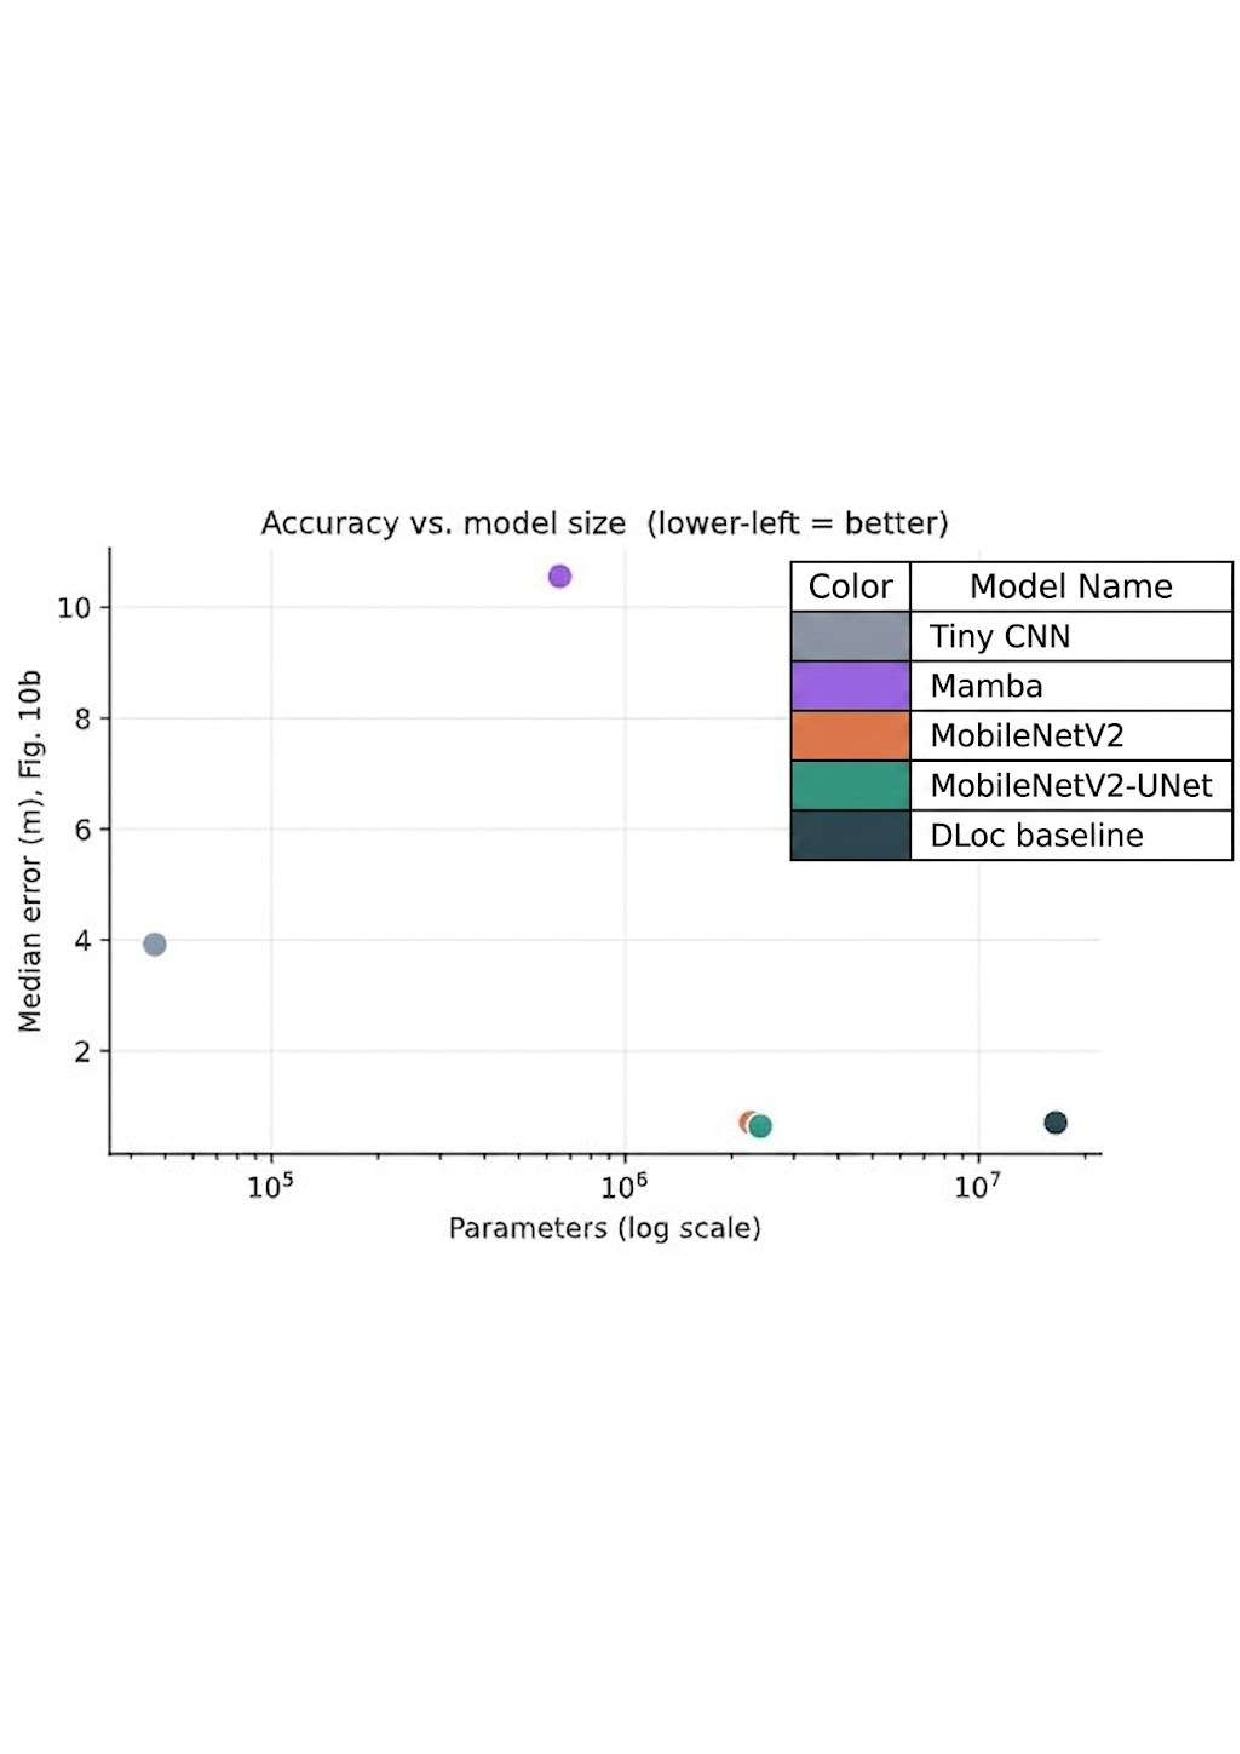
\includegraphics[width=0.92\linewidth]{compression_pareto.pdf}
\caption{Accuracy versus model size. The MobileNetV2-UNet sits at the favorable lower-left of the accuracy--size plane, achieving the best median error among all models at a fraction of the DLoc parameter count.}
\label{fig:pareto}
\end{figure}

\section{Conclusion}
We studied whether DLoc's high computational cost is intrinsic to WiFi localization or an artifact of over-parameterization. Our results show that lightweight models can deliver remarkable localization accuracy while drastically reducing the parameters, computation, and inference time required. A 2.3\,M-parameter MobileNetV2 matches our DLoc reproduction's 0.707\,m accuracy ($7.2\times$ smaller), and a 2.41\,M MobileNetV2-UNet improves it to 0.640\,m---level with DLoc's published median---while using $56\times$ fewer FLOPs and $10\times$ less CPU time, and remaining competitive with DLoc under the same leave-one-session-out protocol.

Beyond raw accuracy, the study yields two design insights. First, knowledge distillation improves robustness rather than in-distribution accuracy, and only for students above ${\sim}2$\,M parameters; below that threshold it harms robustness. Second, architecture and training contribute complementary robustness---skip connections protect best against noise, while distillation protects best against AP dropout. A model an order of magnitude smaller than DLoc can therefore meet or exceed its accuracy, supporting practical WiFi localization on edge devices.

Several directions remain for future work: deploying these networks on edge devices around the E-JUST campus; collecting a new CSI dataset in a different building to test transferability and domain adaptation; adding corruption augmentation during training; extending the statistical validation to the student models; and exploring attention-augmented skip connections and Mamba-style layers.

\nocite{*}

\bibliographystyle{IEEEtran}
\bibliography{references}

\end{document}
